\documentclass[12pt]{article} % For LaTeX2e
\usepackage{nips13submit_e,times}
\usepackage[colorlinks=true, urlcolor=blue]{hyperref}
\usepackage{url}
\usepackage{graphicx}
%\documentstyle[nips13submit_09,times,art10]{article} % For LaTeX 2.09


\title{CSE 6242 Final Project Report}

\author{
Revant Kumar\\
\And
Ashwini Khare\\
\And
Parminder Bhatia\\
\And
Gopi Krishnan Nambiar
}

% The \author macro works with any number of authors. There are two commands
% used to separate the names and addresses of multiple authors: \And and \AND.
%
% Using \And between authors leaves it to \LaTeX{} to determine where to break
% the lines. Using \AND forces a linebreak at that point. So, if \LaTeX{}
% puts 3 of 4 authors names on the first line, and the last on the second
% line, try using \AND instead of \And before the third author name.

\newcommand{\fix}{\marginpar{FIX}}
\newcommand{\new}{\marginpar{NEW}}

\nipsfinalcopy % Uncomment for camera-ready version

\begin{document}

\maketitle

\section{Introduction}

Yelp reviews have been a great source of reviews to customers, which help them choose the best businesses in their region. Currently, if a prospective entrepreneur wants to understand the market scenario, he has to read all the reviews in the region to get an idea about the demand in that region. This strategy is neither feasible nor accurate. 

However, we are looking to provide entrepreneurs trying to set up new business in a particular region with relevant suggestions for establishing a successful business. We aim to make a tool to provide the relevance of features in a particular region. As an example, let's say we are focussing on restaurants in a region. There are various features like hospitality, price, service etc. that make a hotel successful. We aim to provide the relative importance among these features. 

The first problem is that these features are not explicitly provided in the available ratings. We try to solve this problem using Topic Modeling in order to get hold of the inherent features. Once we have these features, we need to find the relative importance of each of the features per business. There are various approaches to this problem. We plan to test these approaches and figure out the best fit. One approach is to take the average for a feature. Another approach is to use Sentiment Analysis to find a relative weight for each feature. 

We plan to start with one city and once we are able to get some useful results, we plan to extend it across 3-4 cities. We will develop the UI for this analysis which would basically be geospatial based and would help prospective businessmen to analyze the regions and which regions match to what services they can offer.

\section{Proposed Method}

\subsection{Data Collection and Normalization}

We have used the review.json and business.json of the Yelp Data-set. The json format of Reviews and Business are as follows:

\begin{figure}[h]
\begin{center}
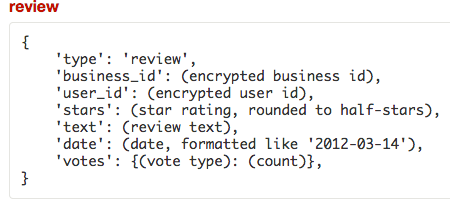
\includegraphics[width=4in]{review.png}
\end{center}
\end{figure}

\begin{figure}[h]
\begin{center}
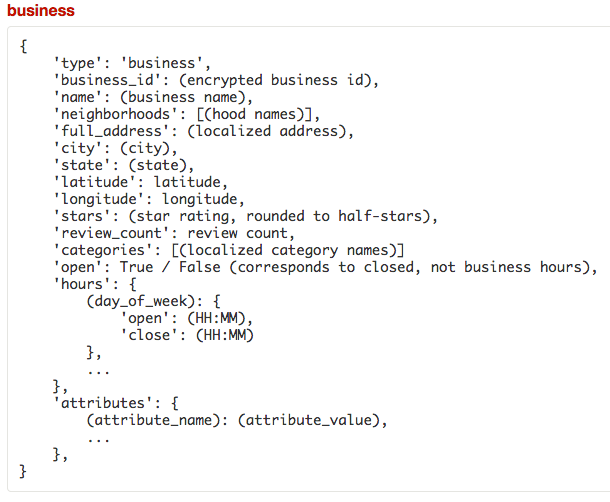
\includegraphics[width=4in]{business.png}
\end{center}
\end{figure}

\subsubsection{Pre Processing of Data}

We extracted the reviews from the json file and imported them to MongoDB in a collection called Reviews. Here as we are dealing with reviews of Restaurants for Phoenix, thus we have applied filtering at this stage to extract relevant reviews.

Now, we loop through all the reviews in the initial dataset and for each review, we split the review into sentences, remove stopwords, extract parts-of-speech tags for all the remaining tokens, filters out all words which are not nouns, uses Lemmatizer/Stemmer to lookup the lemma of each noun. We have used just the Nouns as using other POS were not giving us good topics, that we are interested in. We have also used lemmatizer should as to strengthen words that belong to a single lemma.

Finally, we store each review i.e. reviewId, business name, review text  together with nouns' lemmas to a new MongoDB collection called Corpus.

Following is the output we obtain as words from the text: Refer Figure 1.

\begin{figure}[h]
\begin{center}
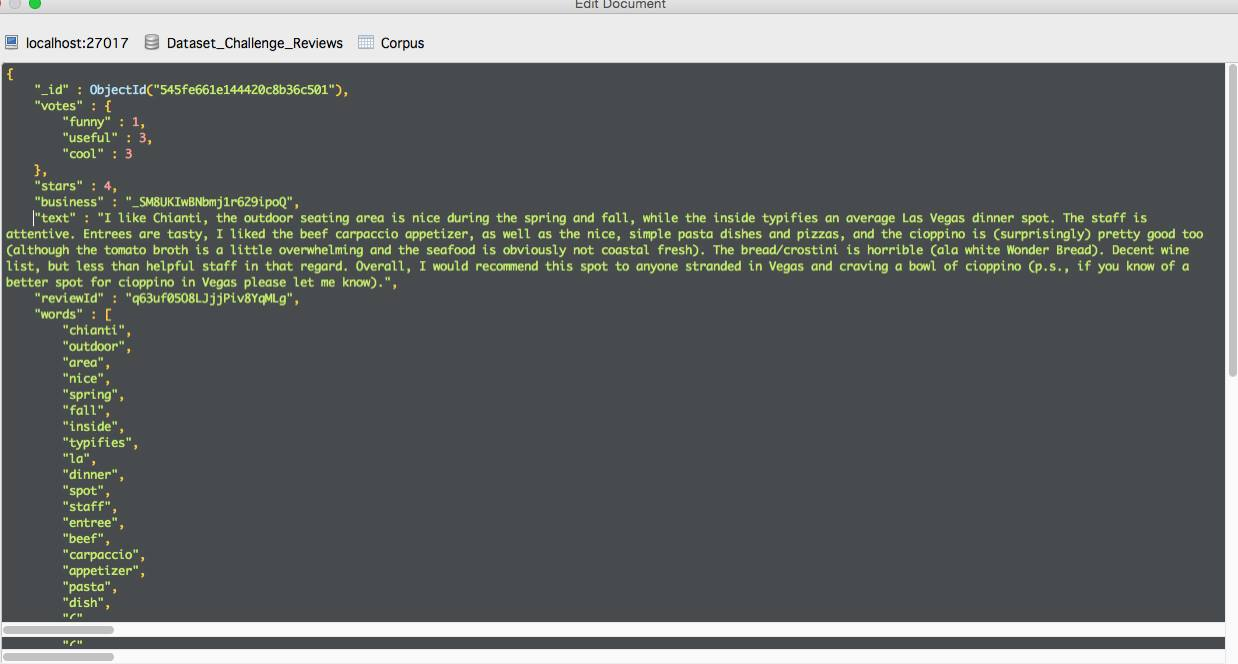
\includegraphics[width=6.5in]{data2.png}
\caption{Output obtained as list of words from the review text}
\end{center}
\end{figure}

\subsection{Online LDA}

Here, we have used Gensim to perform the online LDA on the filtered collections that we have obtained above. We have basically three steps for this process:

\begin{itemize}
\item OnlineLDA : Feeds the reviews corpus created in the previous step to the gensim LDA model. This is a training process which takes number of topics to be generated as input and output for this process are the following:

	\begin{itemize}
	\item Dictionary file: Represents the dictionary structure for the words.
	\item Corpus : This is the output after LDA Algorithm. Corpus is saved in a Market Matrix format as it is a sparse matrix.
	\end{itemize}
	
Further, this is implemented as an Online algorithm, so whenever we add a new review we will update the Dictionary and Corpus based on the review and save the updated files.

\item ShowTopics : Is Responsible for showing the 20 generated topics along with the words within them based on all the reviews.

\item ShowTopicsForReview : Gives us the topics for the review along with their probabilities.

\end{itemize}

\subsection{Latent Topic Rating}

From the above section, we have obtained the latent topics for each of the reviews.

Now, we want to evaluate the average rating of these Latent Topics for a given Business. As, each Business can have multiple reviews, so to obtain the Latent Topics for Business along with their ratings, we combine the latent topics corresponding to each of the reviews belonging to that business and then take average across those topics. 

As an example, lets say Business Domino's had two reviews R1 and R2. R1 had topics Ambience 4, Quality 3 and R2 had topics Service 5, Ambience 3 .Then, topics for Dominos will be Quality with rating 3, Service with rating 5 and Ambience with rating 3.5 ((3+4)/2). 
 
Thus, the above algorithm gave us the Latent Topics of all the Businesses. As, each Business JSON Object also provides us with the pair (Latitude,Longitude), thus now we can easily evaluate the demand and delivery of each of these Latent Topics in the geographical regions of the city.
 
%For calculating the latent topics ratings for topics 
%
%Here we will be incorporating two approaches in order to obtain ratings for the subtopics.
%
%ggregated Ratings-Ratings for a given topic in a Review will be obtained by averages over all of these review ratings to get the hidden topic rating.

%\item In the next approach we will use Multi Aspect Semantic Analysis in order to obtain individual ratings for the Hidden SubTopics in the Review
%\end{itemize}

\subsection{Evaluation}

Our software is live and hosted on \href{http://a.ashwinikhare.in:8030/yelpolo}{http://a.ashwinikhare.in:8030/yelpolo}. 

The screenshot of the webpage can be seen in Figure 2.

\begin{figure}[h]
\begin{center}
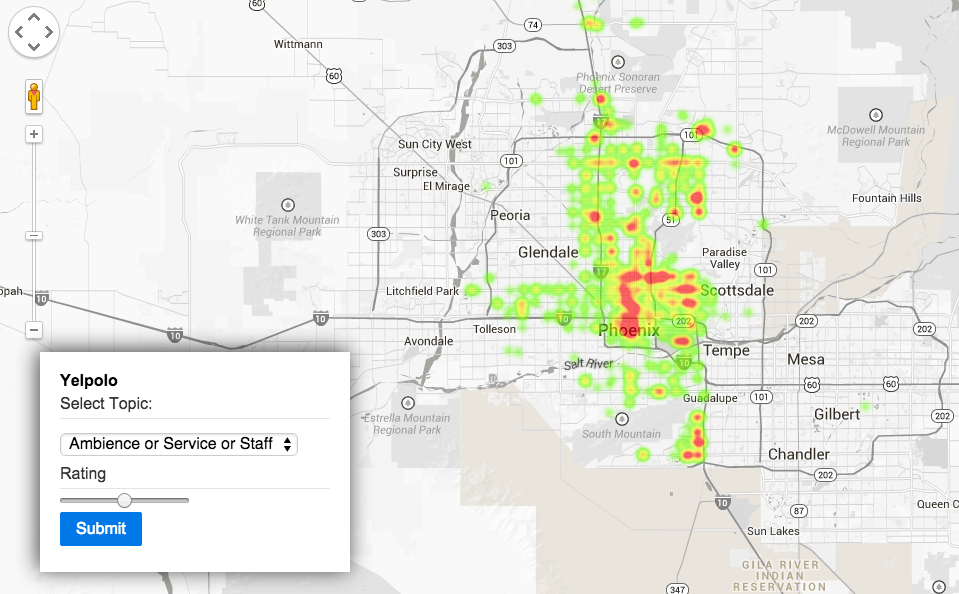
\includegraphics[width=6.5in]{yelp_2.png}
\caption{Webpage of our Software Yelpolo}
\end{center}
\end{figure}

The following are our observations:

\begin{itemize}

\item We have incorporated online LDA. We save our corpus and model using a Sparse Matrix as they are computationally fats and memory efficient. There exist several file formats for serializing a Vector Space corpus (~sequence of vectors) to disk. We did them via the streaming corpus interface. Specifically we used the Blei's LDA-C format. So new reviews can be extended with the existing model by loading and storing these sparse matrix files. Thus, in future if  we wish to enter more dataset, then we can easily extend the existing model.

\item We can determine from the results (Figure 3) that the most important topics found after performing online LDA are the following:

	\begin{itemize}
	\item Ambience
	\item Location
	\item Variety
	\item Wait Time \& Management
	\end{itemize}
	
These topics have the maximum occurrences among the businesses with the average rating in range of 2.5-3.5. Thus, focusing on these aspects can prove successful for the new businesses.

\item We have used Heatmaps along with the Google Map API in order to determine the regions were the businesses will have a higher probability of success. Thus, if the potential user chooses a particular topic from the dropdown and select a particular rating, then the heatmap will show the regions marked with different colors. The regions marked with red correspond to the places where the occurrences of the selected rating are maximum.

Thus, for example, if the user wants to find all the places where a particular aspect has a rating of 2, then he/she can select the aspect from the dropdown and choose the rating of 2. The red color in the heatmap will show all the places in the city where the  occurrence of rating of 2 for that particular aspect is maximum. By this way, the user can identify the places which lack in that particular aspect. So if he/she opens a business along with providing that aspect, then their probability of being successful is higher.

Using this, we found that the central region of Phoenix city has a low rating of Ambience and Service. Thus, if some potential business opens up a restaurant in central Phoenix and provide good ambience and service, then it is likely that his/her business will be more successful.
 
\item Due to some inherent noise in the data, not all words in the subtopic correspond to the inferred meaning.

For example:
	\begin{itemize}
	\item Ambience Or Service or Staff -- 0.105*super + 0.079*place + 0.039*wow + 0.033*food + 0.025*staff + 0.023*hang + 0.021*cheap + 0.013*service + 0.012*time
	
	Here,
		\begin{itemize}
		\item Ambience or Service or Staff is the intuitive name given  to the Topic (by us) based on the words in the topic
		\item super ,place etc are the words in a particular sub-topic 
		\item Numbers correspond to probability of a particular word belonging to the topic.
		\end{itemize}
		
	As , can be seen in the example above , this topic corresponds to more than one topic that can be inferred by a human. example:this topic consists of service and place. This shows that 60 may not be an exact number of subtopics and we should should have gone for slightly more subtopics in the latent space.\\ 
	
	\item Group and Team Outing -- 44: 0.035*pm + 0.027*rail + 0.027*ta + 0.025*brussels + 0.024*remember + 0.023*crepe + 0.023*team + 0.023*event + 0.021*ya + 0.021*waste
	
	This example demonstrates that some noise words can also become part of the topic.
	\end{itemize}


\end{itemize}

\begin{figure}[h]
\begin{center}
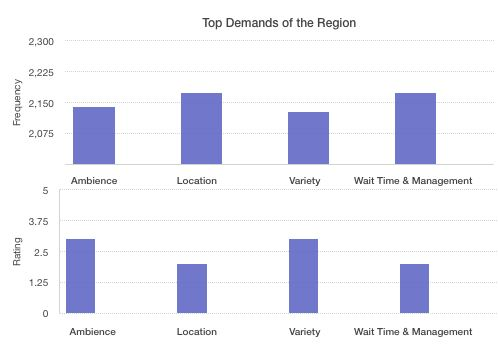
\includegraphics[width=5in]{eval.jpg}
\caption{Top Demands of the region}
\end{center}
\end{figure}

\newpage

\begin{figure}[h]
\begin{center}
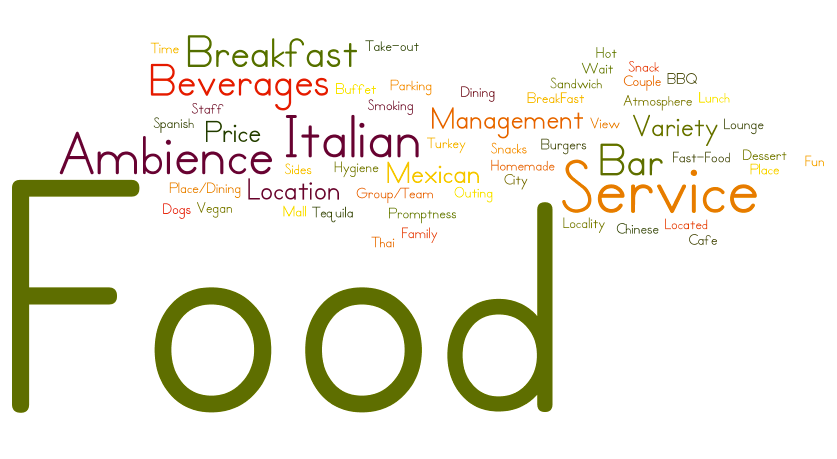
\includegraphics[width=6in]{wordle.png}
\caption{Wordle of the Latent Topics Obtained}
\end{center}
\end{figure}

\subsection{Development of Graphical User Interface}

The graphical user interface is developed using HTML5, CSS3, \& Google Maps API. We have used the heatmaps to visual the regions based of the topics and their ratings. The regions which are shown in red color correspond to the places which the higher occurrence of that selected rating for the topic. The interactions of user is handled using Javascript and a server is sending JSON responses as per user selected filters. 

Our software is live and hosted on \href{http://a.ashwinikhare.in:8030/yelpolo}{http://a.ashwinikhare.in:8030/yelpolo}. 

A screenshot of the UI can be seen in the Figure 5. 

\begin{figure}[h]
\begin{center}
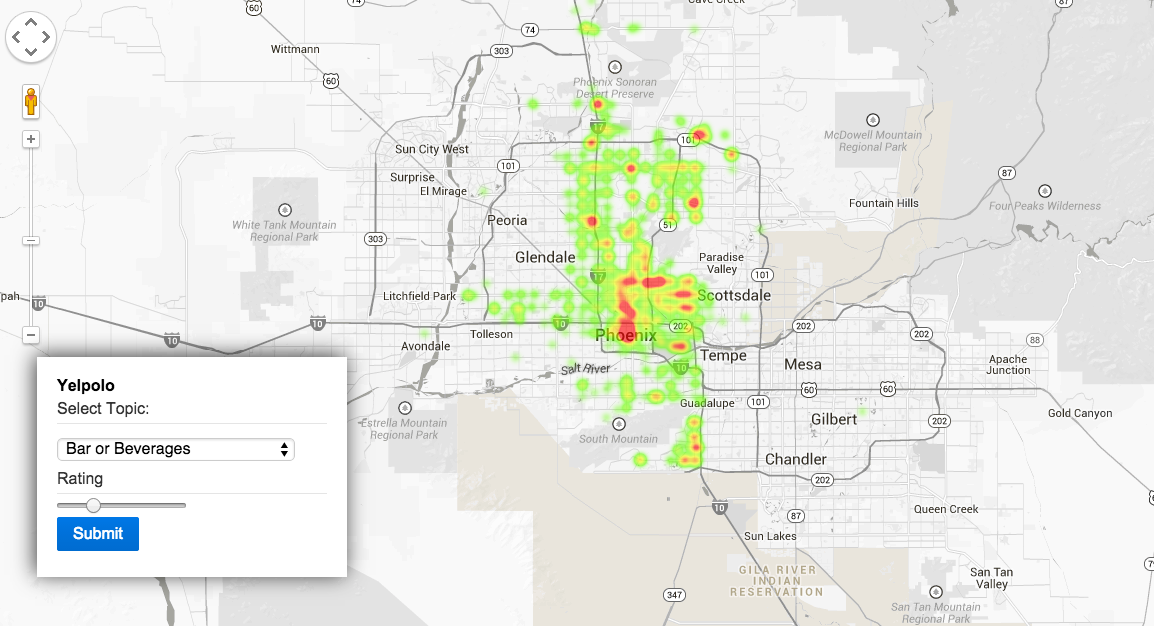
\includegraphics[width=4.8in]{screen.png}
\caption{Yelpolo Webpage}
\end{center}
\end{figure}

The user may require results on various levels of parameters. Thus, we have added filters to the dataset to further enhance the results we generate. Filters are based on the SubTopics and their ratings. The filter looks as shown in the Figure 6.

\begin{figure}[h]
\begin{center}
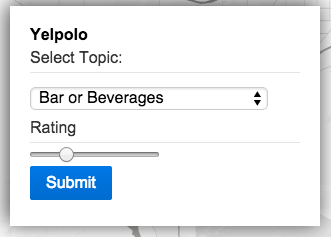
\includegraphics[width=4.8in]{filter.png}
\caption{UI of Filter}
\end{center}
\end{figure}

\subsection{Instructions to Use our Software}

The following are the steps of using our software. We have already provided a screenshot of our interface before in this report. It is hosted on \href{http://a.ashwinikhare.in:8030/yelpolo}{http://a.ashwinikhare.in:8030/yelpolo}.

The steps are:

\begin{itemize}
\item First, the user selects the topic from the drop-down for which he/she wants scan the region.
\item Then, the user uses the bar present on the filter to select a particular rating for that topic. User chooses the particular rating for which he/she wants to identify the regions where the occurrence of this rating is maximum for the already selected topic.
\item Finally, a heat-map is displayed which shows that different regions of the city for that particular topic. Red Color corresponds to the region where the intensity of that rating is maximum as compared to the other regions of the city.
\end{itemize}

\section{Technology Stack}

We will be using the following technologies in our project:
\begin{itemize}
\item Yelp Data Set obtained from their challenge website
\item Python
\item Digital Ocean
\item MongoDB - PyMongo \& RoboMongo
\item Natural Language ToolKit (NLTK)
\item Gensim - Topic Modeling for Humans
\item Git
\item Google Maps API
\end{itemize}

\section{List of innovations}

\textbf{Extracting ratings for the individual sub topics:} Most of the existing reviews today, including the Yelp reviews provide access to a raw rating figure, which is not indicative of the individual sub topics that are rated i.e. ambience, Wi Fi access or speed of service and accessibility. We plan to provide a rating system, which is based on sub topics and the user is able to drill down and search for exactly a particular sub topic that he/she is interested in, without manually going through each of the topics.

\textbf{Helping the entrepreneur with reviews rather than the customer:} Reviews and ratings usually provide a method and system to help the customer figure out the best possible options among the available businesses to choose from. But in our project, we try to help entrepreneurs or the business owners with suggestions on which locality would help them maximize the services that they offer. This project can double up as a recommendation system that matches the services offered by a restaurant with a locality and predicts the optimal locality for the restaurant.


\section{Conclusion}

Thus, in conclusion, we have successfully analyzed the Yelp Dataset to obtain to the hidden topics in the reviews by applying Topic Modeling (Online LDA) and later finding the latent rating of each such topic. Finally, we have also completed the user interface for our software ``Yelpolo'' which displays the intensity of the ratings of the particular topics for the various regions of Phoenix City. Also, we have supported our software with exhaustive evaluations as explained before in the report.

Thus, we believe that our software can help the potential businessmen to find the places where the success of opening their business has a higher probability as compared to the other regions of the city. 

For the future work, we feel that the latent topic ratings can be improved by using Multi-Aspect Sentiment Analysis. Also, this approach can also be used to find similarity between business based on latent topics. Thus, the input matrix could be fed into any clustering algorithm to find the business which provide similar type of subtopics.

\section{Appendix}

\subsection{Appendix A: Plan of Activities}

Refer the table.

\begin{figure}[h]
\begin{center}
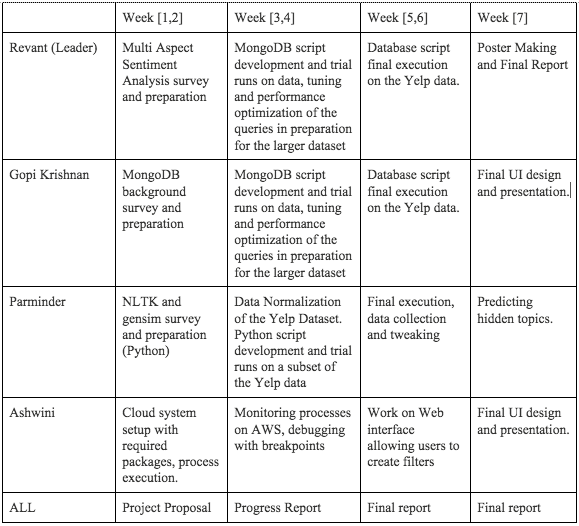
\includegraphics[width=6in]{act.png}
\end{center}
\end{figure}

\subsection{Appendix B: Distribution of team member effort}

All team members contributed an equal amount of effort to the project.

\subsection{Appendix B: Survey with Categories}

\subsubsection{Topic Modeling}

\paragraph{Improving Restaurants by Extracting Subtopics from Yelp Reviews}
This is the main paper for our project. This paper used LDA for topic modeling to find various topics in reviews. Weights for features selected is quite simplistic based on the weighted average. This paper considers only a single city dataset and lacks any UI in order to infer results. They do not consider fraud detection in reviews.

\paragraph{Spatial Topic Modeling in Online Social Media for location Recommendation}
The publication was one of the first attempt to consider the user, the post and the location for topic modeling by creating a spatial topic model. The methodology used in development of the model, ie, MCEM method to learn latent variables is a part of one of our experiments for it maximizes the likelihood of observed random variables. A limitation of this model is that others ignored certain aspects like the ratings of the review.

\paragraph{Hidden Factors and Hidden Topics: Understanding Rating Dimensions with Review Text} 
Authors have tried to improve the prediction of how a user will respond to a new product when it is recommended to the user. This can be improved by considering the user's tastes along with the properties of each product. They have presented a model called HFT combining ratings with review text for recommendations. We will modify this to give geographical recommendations, so that the users get an idea of places where a businesses can be opened successfully. 

\subsubsection{Rating Prediction}

\paragraph{Multi-aspect Sentiment Analysis with Topic Models}
Authors have tried to look beyond the aggregated ratings of reviews and have investigated the role of LDA to Multi-Aspect Sentiment Analysis tasks to take into account related aspects often discussed within a single review. The approach used will help us to give ratings and aspect-based review summarization for each of the latent topics.

\paragraph{Your Neighbors Affect Your Ratings: On Geographical Neighborhood Influence to Rating Prediction}
This paper studies the impact of the neighbourhood on the Yelp ratings of a business by making use the check in records of the users. Each business is modeled with two vectors of latent factors, one for the quality of the business and the other for the influence of its neighbourhood characteristics.We propose to perform sentiment analysis of the reviews and use it in our project in order to predict an optimal location where a business can be set up, which is a shortcoming of the current approach

\subsubsection{Yelp Reviews}

\paragraph{Online Word of Mouth: Characteristics of Yelp.com Reviews}
In this publication the author draws a comparison of electronic form of communication compared to the traditional one by experimenting on yelp dataset and categorizing results. A possible useful result of the experiment was how readers were indifferent to the length of the review. The author ignored various dimensions of data and test sample was too small.

\subsubsection{UI Design}

\paragraph{Clustered Layout Word Cloud for User Generated Review}
Objective of this paper was that the word cloud needs to use its layout to present semantic information and the word cloud needs to support interaction for retrieval of review content.Force-directed graph layout is a good model for performing the clustering process in our word cloud design and different clusters can be colored differently based force directed graph layout. This paper provided insights on how we plan to visualize our results using clustering of word clouds and using force directed graphs.

\subsubsection{Fake Detection}

\paragraph{What Yelp Fake Review Filter Might Be Doing}
This paper showed that behavioral features significantly outperform Linguistic n-grams on detection performance. Classification under balanced class distribution gives an accuracy of significantly higher than random guessing. They show that fake review detection using linguistic features is not so effective in the real-life setting, and crowdsourced fake reviews may not be representative of real-life fake reviews. Helps in understanding yelp review systems and their filter which gives us scope to apply clustering based on these criteria as well as apply and enhance traditional linguistic fraud detection techniques on the data set. 

\paragraph{Opinion Fraud Detection in Online Reviews by Network Effects} 
This paper proposes an unsupervised learning method to detect fraudulent reviews in online platforms based on signed bipartite graphs, sentiment analysis and probabilistic models for classification. However, using this approach, the fraud detection algorithm is based more on behavioral features and hence it is likely to underperform on the Yelp dataset that we are using.

\subsubsection{Recommendations}

\paragraph{Recommendation via user's personality and social context}
In this work, the authors primarily devise a personalized recommendation system by adding a component of personal interest, interpersonal interest similarity and interpersonal influence. For our utility, we make use of the results of their probabilistic factorization model and how to increase relevance of results. The drawbacks in their approach were that they only considered past rating history data and ignored the location dimension.

\paragraph{Generating Recommendation Dialogs by Extracting Information from User Reviews} 
Authors have presented a framework for generating and ranking fine-grained, highly relevant questions from user-generated reviews helping users to navigate e-commerce listings by asking questions about users' preferences toward domain attributes. This helps us to ask questions specific to the business that user is looking to open so that we can predict the best geographical locations where the user's business is successful.

\paragraph{Discovering contextual information from User reviews for Recommendation purposes}
This paper describes an approach to figure out context related information from the user generated reviews by separating the user reviews into generic and specific types. Both word based and LDA based methods capture relevant contextual data in a user review. This paper describes a very efficient method of extracting contextual information from the user reviews which can be treated as an input to our program.

\section{References}
\begin{itemize}
\item Improving Restaurants by Extracting Subtopics from Yelp Reviews: J Huang, S Rogers, E Joo - 2014 - ideals.illinois.edu
\item What Yelp Fake Review Filter Might Be Doing: A Mukherjee, V Venkataraman, B Liu, NS Glance - ICWSM, 2013 - aaai.org
\item Clustered Layout Word Cloud for User Generated Review: J Wang, J Zhao, S Guo, C North - yelp.co.nz
\item Online Word of Mouth: Characteristics of Yelp.com Reviews: Tiana Tucker - Elon Journal of Undergraduate Research in Communications
\item Recommendation via user's personality and social context: H Feng, X Qian - Proceedings of the 22nd ACM international conference
\item Spatial Topic Modelling in Online Social Media for location Recommendation:  Bo Hu, Martin Ester - RecSys '13  Proceedings of the 7th ACM conference on Recommender systems
\item Hidden Factors and Hidden Topics: Understanding Rating Dimensions with Review Text: J McAuley, J Leskovec - Proceedings of the 7th ACM conference on , 2013 - dl.acm.org
\item Generating Recommendation Dialogs by Extracting Information from User Reviews: K Reschke, A Vogel, D Jurafsky - ACL (2), 2013
\item Multi-aspect Sentiment Analysis with Topic Models: 2011 IEEE 11th International Conference on Data Mining Workshops (ICDMW)
\item Your Neighbors Affect Your Ratings: On Geographical Neighborhood Influence to Rating Prediction: L Hu, A Sun, Y Liu  Proceedings of the 37th International ACM SIGIR conference on Research \& Development in information retrieval
\item Discovering contextual information from User reviews for Recommendation purposes: K Bauman, A Tuzhilin - 2014 - ceur-ws.org
\item Opinion Fraud Detection in Online Reviews by Network Effects: L Akoglu, R Chandy, C Faloutsos - ICWSM, 2013
\end{itemize}

\end{document}